\documentclass[conference]{IEEEtran}
\IEEEoverridecommandlockouts
% The preceding line is only needed to identify funding in the first footnote. If that is unneeded, please comment it out.
\usepackage{cite}
\usepackage{amsmath,amssymb,amsfonts}
\usepackage{algorithmic}
\usepackage{graphicx}
\usepackage{textcomp}
\usepackage{xcolor}
\newcommand{\mycomment}[1]{}
%\usepackage{graphicx}
\usepackage{subcaption}


\def\BibTeX{{\rm B\kern-.05em{\sc i\kern-.025em b}\kern-.08em
    T\kern-.1667em\lower.7ex\hbox{E}\kern-.125emX}}
\begin{document}

\title{Deliverable 5.3.1\\

\vspace{10pt}
\footnotesize{EE0009445 Modeling the Integration of Marine Energy into Microgrids}
}

\maketitle

\section{Deliverable 5.3.1}

\textbf{Report on a test system microgrid stability study with
the developed power converter and system fault-protection
model.}



\subsection{Introduction}



The inherent intermittency of renewable energy resources poses significant challenges to modern electricity grids, particularly at higher penetration levels. To address these challenges, modern grid codes specify stringent connection requirements for new power plant integrations [1]. These requirements encompass power quality standards, including limits on voltage and frequency variations, as well as Fault Ride-Through (FRT) or Low Voltage Ride-Through (LVRT) capabilities during grid faults. Grid codes have evolved to accommodate the increasing penetration of renewable energy sources into existing grids. For instance, a comprehensive review of wind farm grid connection requirements across various countries is presented by [2]. Fig. 1 illustrates the LVRT requirements specified in the  grid codes [1], which mandate that renewable energy power plants remain connected to the grid during and after voltage sags. During fault conditions, renewable power plants must endure voltage dips to a specified percentage of the nominal voltage for a defined time duration.\\

The impact of connecting Wave Energy Conversion Systems (WECS) to microgrids or distribution networks from an electrical and control perspective remains insufficiently explored, indicating a need for a more comprehensive investigation. Previous studies, such as [3], [4], and [5] have focused on grid-connected WECS stability analysis. However, these studies lack detailed electrical and control system insights. Moreover, active distribution networks require further testing under high-penetration offshore WECS with varying operating conditions to examine potential issues such as overvoltage, undervoltage, and frequency excursions — aspects that are currently underexplored in existing WECS literature.\\

To meet the deliverable requirements, a coordinated control scheme integrating LVRT capability for the WEC system is developed. Additionally, a control system is implemented to enhance power quality when the WEC system is connected to an unbalanced network. The impact of integrating variable power WECs on distribution system voltage and frequency parameters is thoroughly examined to assess system stability. The findings of this study are applicable to large microgrids; however, for smaller microgrids, a more detailed analysis focusing on the transient stability of the microgrid's generators and system frequency is required. This aspect is currently under investigation.\\
\begin{figure}[ht]
\centerline{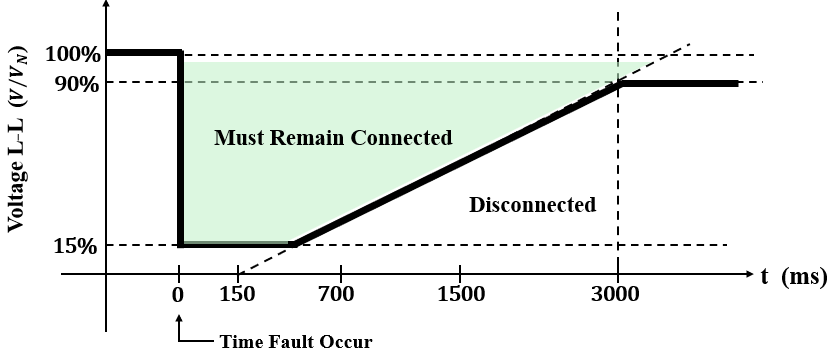
\includegraphics[width=0.5\textwidth]{Figs/5_3_1/lvrt_limit.png}}
\vspace{-0.8em}
\caption{Voltage profiles of LVRT requirement}
\label{fig1}
\end{figure}

\section{WEC Hydrodynamics in WEC-Sim}
This study considers a two-body RM-3 point absorber WEC consisting of a float and a spar. Fig. 2 depicts the high-level diagram of the W2G system. The WEC transforms hydrodynamic forces ($F_{hydro}$) into mechanical force ($F_{PTO}$), which the linear permanent magnet generator (LPMG) then converts into electrical energy. The power conditioning blocks adjust the electrical energy for grid connection.\\
Modeling WEC dynamics in WEC-Sim encompasses the interaction among incident waves, device motion, the power take-off (PTO) mechanism, and mooring. This study uses a LPMG as the direct-drive PTO, with its rotor, known as translator rigidly connected to the WEC. The heave motion of the WEC drives the translator of the LPMG.\\
The dynamic response in WEC-Sim uses Cummin's equation to solve the equation of motion for each body about its center of gravity. The motion equation is 
\begin{equation}
m\ddot{y} = -A_{\infty} \ddot{y} - \int_{0}^{t} K(t-\tau) \dot{y} \, d\tau + F_e + F_v + F_{pto} + F_{res} + F_m
\end{equation}
where $A_{\infty}$ is the added mass at infinite frequency, $m$ is the total mass of the body, $K$ is the impulse response function, $F_e$, $F_{pto}$, and $F_v$ are wave excitation force, PTO force, and viscous drag force respectively, while $y$, $\dot{y}=v$, and $\ddot{y}$ represent relative heave displacement, velocity, and acceleration. 
The first two terms on the right-hand side of Cummin's equation form the radiation force that depends on the body's acceleration and speed. WEC-Sim solves the 



\begin{figure*}[ht]
    \centering
    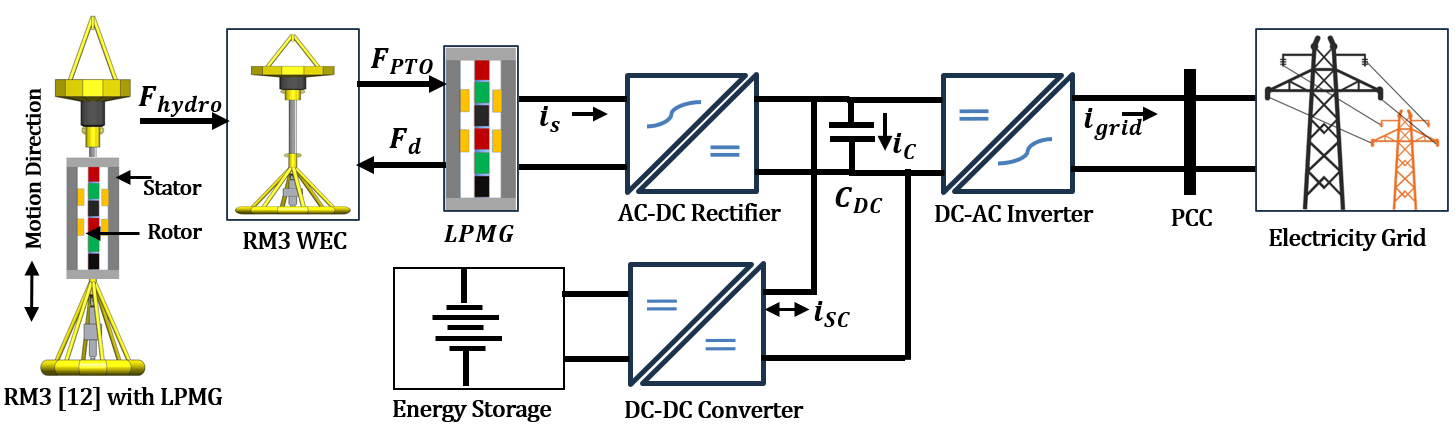
\includegraphics[width=\textwidth]{Figs/5_3_1/block dia2.png}
    \vspace{-2em}
    \caption{Overview of the WEC-to-Grid system.}
    \label{fig:your-label}
\end{figure*}




governing equations of motion in six degrees of freedom $-$ namely
surge, sway, heave, roll, pitch, and yaw $-$ for each body to conduct time-domain simulations.

\section{Synchronous LPMG with GEN- Side Converter}
The rotor of the LPMG reciprocates from its equilibrium position, indicating a change in motion direction, in contrast to the rotary motion of the permanent magnet synchronous generator. Two sets of dynamic equations are proposed in [7] to incorporate the positive and negative direction of motion.
The Park ($dq0$) transformation can help change a balanced three-phase system into a dynamic two-phase system. The reference angle ($\theta$) for the $dq0$ transformation of the LPMG model depends on the translator's displacement which is:

\begin{equation}
\theta = \frac{2\pi}{\tau}y - \frac{\pi}{2}
\end{equation}

Given the positive and negative motion of the translator, the state-space dynamic model of the LPMG with an active rectifier can be written as:
%\vspace{-0.2em}
\begin{equation}
\begin{bmatrix}
\frac{di_{s,d}}{dt} \\
\frac{di_{s,q}}{dt} \\
\frac{dy}{dt}
\end{bmatrix}
=
\begin{bmatrix}
-\frac{| \omega |}{\omega} \frac{R_{eq}}{L_{eq}} & \frac{| \omega |}{\omega} \frac{X_{eq}}{L_{eq}} & 0 \\
-\frac{| \omega |}{\omega} \frac{X_{eq}}{L_{eq}} & -\frac{| \omega |}{\omega} \frac{R_{eq}}{L_{eq}} & \frac{| \omega |}{\omega} \frac{\lambda_m}{L_{eq}} \\
0 & 0 & \frac{\tau}{2\pi}
\end{bmatrix}
\begin{bmatrix}
i_{s,d} \\
i_{s,q} \\
\omega
\end{bmatrix}
\end{equation}
\[
+
\begin{bmatrix}
-\frac{| \omega |}{\omega} \frac{1}{L_{eq}} & 0 \\
0 & -\frac{| \omega |}{\omega} \frac{1}{L_{eq}} \\
0 & 0
\end{bmatrix}
\begin{bmatrix}
v_{s,d} \\
v_{s,q}
\end{bmatrix}
\]
where $v_{s,(dq)}$, $i_{s,(dq)}$ are $d-$ and $q$-axis stator voltages and currents. $L_{eq} = L_s + L_f$, $R_{eq} = R_s + R_f$, $L_f$, $R_f$ are generator-side filter inductance and resistance, $X_{eq} = |\omega| L_{eq}$, and $\omega = \frac{2\pi v}{\tau}$ is the angular frequency of the stator variables.\\

The linear generator exerts a damping force on the floater of the WEC. The damping force $F_d$ controls the movement of the WEC. For a simple non-salient LPMG, where $d-$ and $q-$axis inductances are equal, i.e., $L_{s,d} = L_{s,q} = L_s$, $F_d$ can be written as
\begin{equation}
F_d = \frac{3}{2} \frac{2\pi}{\tau} \lambda_m i_{s,q}
\end{equation}

The damping force is proportional to $i_{s,q}$. The $F_d$ can be made equal to $F_{pto}$ by controlling the $i_{s,q}$, thus forcing the WEC to move in resonance with the incident waves. This resonance ensures the maximum power extraction from wave resources. Hence, $i_{s,q}^{ref}$ for the generator-side converter can be found as
\begin{equation}
i_{s,q}^{ref} = \frac{(-B_w \dot{y} - k_s y) \tau}{3\pi \lambda_m}
\end{equation}

On the other hand, $i_{s,d}^{ref}$ is set to zero to minimize the copper losses of the LPMG. 

\section{Supercapacitor-based Energy Storage and DC-DC Converter}
The intermittent wave force causes the direct drive LPMG's output power and terminal voltage to fluctuate significantly. It is not permissible to add this highly fluctuating power to the grid to maintain power quality and comply with the grid codes. Therefore, an intermediate power smoothing device becomes crucial between the grid-side and generator-side power conditioning units. In this study, a supercapacitor (SC) based short-term energy storage device addresses this power quality issue.
A DC-DC converter connects this SC to the DC link. In discharge mode, the SC supplies power to the DC link, and the converter functions as a Boost converter. Conversely, when power flows from the DC link to the SC, the DC/DC converter operates in Buck mode, thereby charging the SC. 
The DC-link voltage regulation at a nominal level is essential to support the operating conditions of the grid-side inverter. Fig. 3 shows the controller for the DC-DC converter that keeps the DC-link voltage within the nominal range.
\vspace{-1.5em}
\begin{figure}[hp]
\centerline{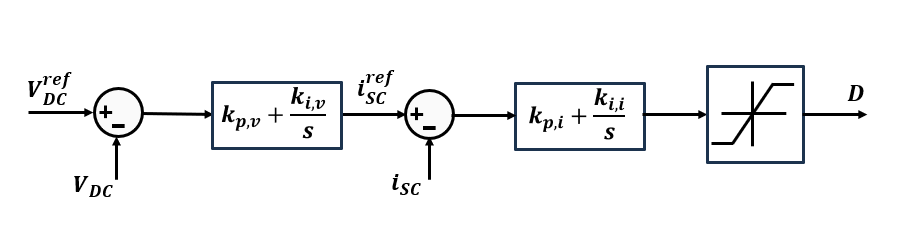
\includegraphics[width=0.5\textwidth]{Figs/5_3_1/dc dc con.png}}
\vspace{-1em}
\caption{DC-DC converter control diagram}
\label{fig1}
\end{figure}

\section{Modeling and Control of Grid-Side Converter}
The grid-side power conditioning unit is a three-phase, three-leg, two-level grid-following inverter (GFLI) with two switches per leg. An RL filter connects the GFLI's AC side to the grid. The DC side is attached to the DC-link capacitor. The dynamic model of the AC side of the inverter in the $abc$-reference frame is
\begin{equation}
\frac{di_{g(abc)}}{dt} = \frac{1}{L_{f,g}} \left( v_{inv(abc)} - R_{f,g} i_{g(abc)} - v_{g(abc)} \right)
\end{equation}

Under normal balanced grid conditions, a Synchronous Reference Frame Phase-Locked Loop (SRF-PLL) can accurately extract the frequency and phase angle from the three-phase grid voltage. By utilizing the PLL, the d-axis component of the grid voltage is aligned with the grid voltage space vector, resulting in a q-axis component of zero. The Park transformation is employed to convert three-phase AC quantities into two DC components, facilitating easier implementation in controller design. However, during unbalanced grid conditions or asymmetrical grid faults, the Park transformation introduces double-frequency oscillations in the d-q components of the grid voltage. Fig. 4 (a) and (b) illustrate the decomposition of d and q components under both balanced and unbalanced grid voltage conditions.

\begin{figure}[h!]
    \centering
    \begin{subfigure}[b]{0.45\textwidth}
        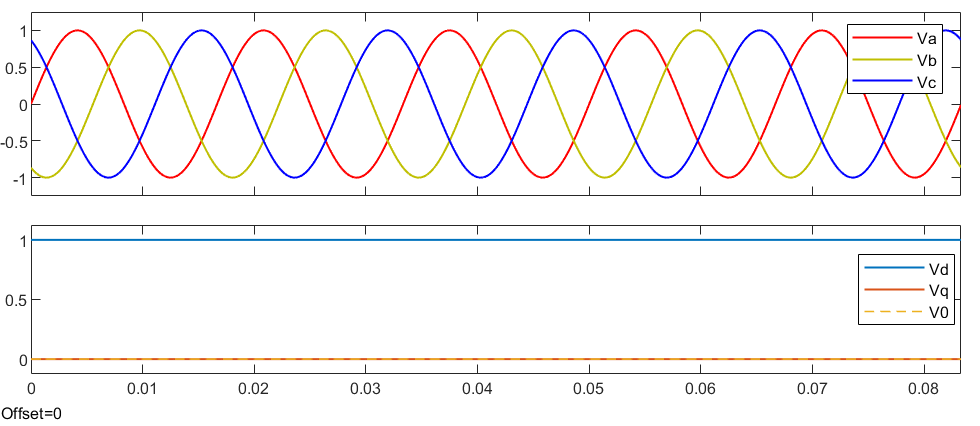
\includegraphics[width=\textwidth]{Figs/5_3_1/vabc_vdq_balance.png}
        \label{fig:a}
    \end{subfigure}
    \hfill
    \begin{subfigure}[b]{0.45\textwidth}
        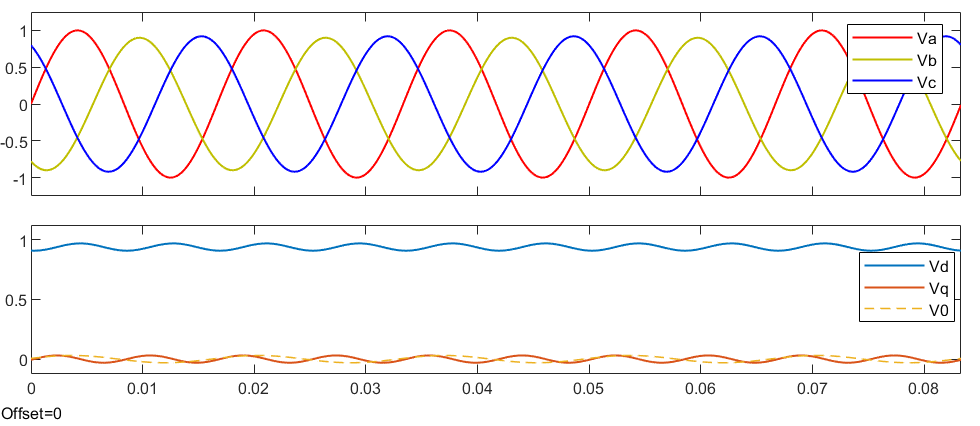
\includegraphics[width=\textwidth]{Figs/5_3_1/vabc_vdq_unbalance.png}
        \label{fig:b}
    \end{subfigure}
    \caption{Decomposition of d and q components under (a) balanced and (b) unbalanced grid voltage conditions.}
    \label{fig:combined}
\end{figure}

The instantaneous real and reactive power also becomes oscillatory in case of unbalanced grid conditions. The oscillation in the active power output creates double frequency oscillations on the DC-link capacitor voltage, which leads to instability of the grid side converter. The instantaneous current out of the inverter for unbalanced grid conditions also becomes unbalanced, which compromises the quality of output power.  
Any unbalanced voltage vector can be expressed as:

\begin{equation}
V = V^+ + V^- + V^0
\end{equation}

\begin{equation}
= V_m^p \begin{bmatrix} \sin(\omega t + \theta^p) \\ \sin(\omega t + \theta^p - 120^\circ) \\ \sin(\omega t + \theta^p + 120^\circ) \end{bmatrix} + V_m^n \begin{bmatrix} \sin(\omega t + \theta^n) \\ \sin(\omega t + \theta^n + 120^\circ) \\ \sin(\omega t + \theta^n - 120^\circ) \end{bmatrix} +\end{equation}
\[
 V_m^0 \begin{bmatrix} \sin(\omega t + \theta^0) \\ \sin(\omega t + \theta^0) \\ \sin(\omega t + \theta^0) \end{bmatrix}
\]




For a 3-phase, 3-wire inverter, the current flowing through phases does not have a zero-sequence component. Therefore, the current vector can be expressed as:

\begin{equation}
I = I^+ + I^- 
\end{equation}

%\begin{equation}
\[
= I_m^p \begin{bmatrix} \sin(\omega t + \phi^p) \\ \sin(\omega t + \phi^p - 120^\circ) \\ \sin(\omega t + \phi^p + 120^\circ) \end{bmatrix} + I_m^n \begin{bmatrix} \sin(\omega t + \phi^n) \\ \sin(\omega t + \phi^n + 120^\circ) \\ \sin(\omega t + \phi^n - 120^\circ) \end{bmatrix}
\]
%\end{equation}


These three quantities of every sequence can be transformed into two quantities using the Clarke and Park transformation. The instantaneous three-phase real and reactive power for unbalanced voltage conditions can be written as
\begin{equation}
\begin{bmatrix} p \\ q \end{bmatrix} = \begin{bmatrix} \overline{P} \\ \overline{Q} \end{bmatrix} + \begin{bmatrix} \tilde{p} \\ \tilde{q} \end{bmatrix} = \begin{bmatrix} \overline{P} \\ \overline{Q} \end{bmatrix} + \begin{bmatrix} P_{c2} \\ Q_{c2} \end{bmatrix}\cos(2\omega t) + \begin{bmatrix} P_{s2} \\ Q_{s2} \end{bmatrix}\sin(2\omega t)
\end{equation}

Where, $\overline{P}$ and $\overline{Q}$ are the average components, and $\tilde{p}$ and $\tilde{q}$ represent the oscillatory components of real and reactive power. The average and oscillatory terms can be derived from the dq-components of the positive and negative sequence voltages and currents as follows:

\begin{equation}
\begin{bmatrix} \overline{P} \\ \overline{Q} \\ P_{c2} \\ P_{s2} \\ Q_{c2} \\ Q_{s2} \end{bmatrix} = \begin{bmatrix} v_d^p & v_q^p & v_d^n & v_q^n \\ v_q^p & -v_d^p & v_q^n & -v_d^n \\ v_d^n & v_q^n & v_d^p & v_q^p\\ v_q^n & -v_d^n & -v_q^p & v_d^p \\v_q^n & -v_d^n & v_q^p & -v_d^p \\ -v_d^n & -v_q^n & v_d^p & v_q^p \end{bmatrix} \begin{bmatrix} i_d^p \\ i_q^p \\ i_d^n \\ i_q^n \end{bmatrix}
\end{equation}

Where,

\begin{align*}
v_d^p &= V_m^p \cos(\theta^p), & v_q^p &= V_m^p \sin(\theta^p), \\
v_d^n &= V_m^n \cos(\theta^n), & v_q^n &= -V_m^n \sin(\theta^n), \\
i_d^p &= I_m^p \cos(\phi^p), & i_q^p &= I_m^p \cos(\phi^p), \\
i_d^n &= I_m^n \cos(\phi^n), & i_q^n &= -I_m^n \cos(\phi^n).
\end{align*}

It can be observed from the equation that there are four variables ($i_d^p$, $i_q^p$, $i_d^n$, $i_q^n$) to control six quantities ($\overline{P}$, $\overline{Q}$, $P_{c2}$, $P_{s2}$, $Q_{c2}$, $Q_{s2}$). Typically, for grid-connected operation, a certain $\overline{P}$ and $\overline{Q}$ need to be injected. Thus, for a three-phase, three-wire inverter, with a specified amount of average $P$ and $Q$ grid injection, the remaining two quantities out of the four can be controlled using the four control variables.
The imbalance in the inverter output current can be eliminated using a dual sequence controller by making $i_d^n = i_q^n = 0$. Thus, for an unbalanced grid, with a particular average $P$ and $Q$ injection, the current references of the Grid-SC controller become:

\begin{align}
i_{d,ref}^p &= \frac{2(v_d^p \overline{P} + v_q^p \overline{Q})}{3((v_d^p)^2 + (v_q^p)^2)} \\
i_{q,ref}^p &= \frac{2(v_q^p \overline{P} - v_d^p \overline{Q})}{3((v_d^p)^2 + (v_q^p)^2)} \\
i_{d,ref}^n &= i_{q,ref}^n = 0
\end{align}

However, making the negative sequence component zero from the output Grid-SC current doesn’t eliminate the oscillatory components $P_{c2}$, $P_{s2}$, $Q_{c2}$, and $Q_{s2}$. Consequently, oscillations will persist in the output active and reactive power.
\subsection{LVRT and Current Limitation Control Strategy}
During low voltage, grid code requires the inverter to ride through the voltage for a certain amount of time and also to inject reactive power to support the grid voltage. The US grid code requires the inverter to inject the following reactive current during a fault
\begin{equation}
i_{q}^{p} = \begin{cases} 0 & \text{if } \frac{v_d^p}{v_{nominal}} > 0.9 \\ 2 \times \left(1 - \frac{v_d^p}{v_{nominal}}\right) \times i_n & \text{if } 0.5 < \frac{v_d^p}{v_{nominal}} \leq 0.9 \\ i_n & \text{if } \frac{v_d^p}{v_{nominal}} < 0.5 \end{cases}
\end{equation}

However, the inverter has a certain current limit that depends on the current rating of the switching device. The current space vector can be expressed as:

\begin{equation}
I^2 = 
\end{equation}\[
(I^p)^2 + (I^n)^2 + 2 \times I^p \times I^n \times \cos\left(\tan^{-1}\left(\frac{i_q^p}{i_d^p}\right) + \tan^{-1}\left(\frac{i_q^n}{i_d^n}\right)\right)\]
%\end{equation}

Where,

\begin{align*}
I^p &= \sqrt{(i_d^p)^2 + (i_q^p)^2}, \\
I^n &= \sqrt{(i_d^n)^2 + (i_q^n)^2}
\end{align*}

During a fault, $i_q^p$ is determined by the grid code. The rest of the three current references need to be selected in a way that limits the inverter's maximum current limit.\\

In normal operation, the active power reference $\overline{P}$ in the equation (12)-(13) is the average power generated by the WEC. However, during a fault, the active power reference needs to be reduced from the generated average power so that the inverter current limit is not violated. To determine the active power reference during a fault, an online current limiting strategy is employed.

\\
For dynamically varying generated power from WEC, the injected grid current amplitude also varies with time. To immediately release the energy stored from the supercapacitor into the grid without exceeding the inverter current limit, the recovery time, $t_{rec}$ is selected as follows:

\begin{equation}
t_{rec} = \frac{E_{rec}}{P_{max} - \overline{P}}
\end{equation}

Where,

\begin{equation}
E_{rec} = \int_{t_{fs}}^{t_{fe}} (P_{gen} - \overline{P})\, dt
\end{equation}

\section{Simulation Results and Discussions}
The W2G system is implemented in MATLAB/Simulink. First, the performance of the dynamic W2G system is evaluated in the normal grid condition. Then the performance is evaluated during the grid fault. Three-phase symmetrical voltage dips are considered for assessing the LVRT performance. A strong grid condition is assumed while evaluating the LVRT performance. Then, the W2G system is connected to a remote bus of the IEEE 13-node distribution test case, and the effect of connecting the variable power wave energy on the distribution system is investigated. Voltage and frequency disturbances are applied to the 13-bus system to evaluate the transient behavior of the W2G system.
\subsection{Normal Grid Condition}
Fig. 5-8 shows the W2G system performance in normal grid conditions. The position and velocity of LPMG’s translator are varying irregularly for an irregular wave condition. The $i_{qs,ref}$ for the Gen-SC is determined to make the WEC movement in resonance with the incoming wave force so that maximum power can be extracted. The Gen-SC perfectly controls the d- and q-axis currents to its reference value, as shown in Fig. 5. The SC controls the DC-link capacitor voltage and helps to smooth out the generated power ripple. The DC-DC converter’s performance is shown in Fig. 6 where the DC bus voltage is perfectly maintained to its reference level. A low-pass filter (LPF) is used to filter out the fluctuations of generated power from the LPMG. The LPF is implemented in the control system of Gen-SC. The Grid-SC is controlled to inject the filtered power into the grid while maintaining zero reactive power during normal grid conditions. Fig.7 shows the real and reactive power injection into the grid by the Grid-SC, which perfectly tracks the real and reactive power references.
\begin{figure}[htbp]
    \centering
    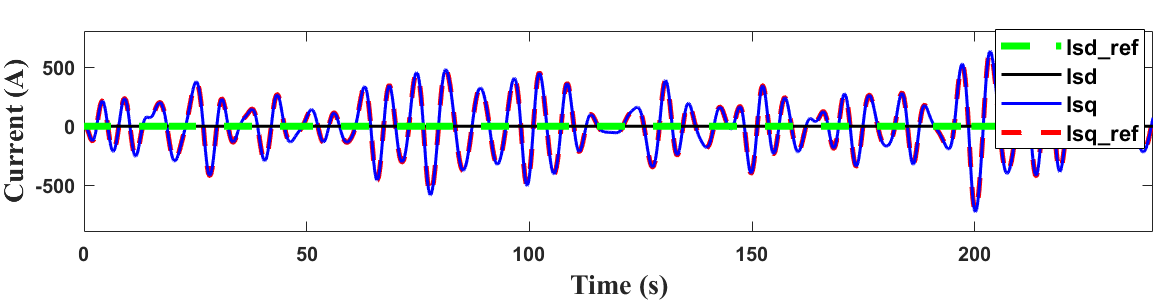
\includegraphics[width=0.5\textwidth]{Figs/5_3_1/gen current.png}
    \caption{d- and q- axis current tracking of Gen-SC}
    \label{fig:W2G_normal_grid}
\end{figure}
\begin{figure}[h!]
    \centering
    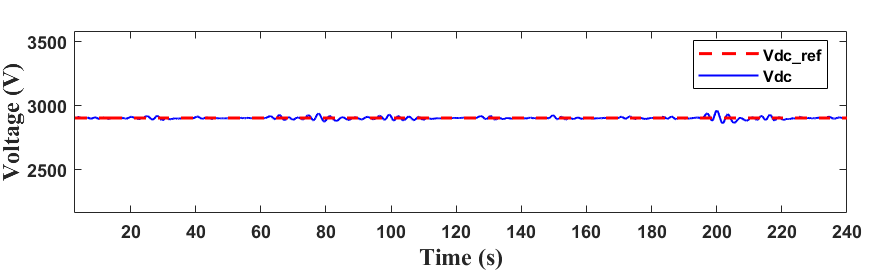
\includegraphics[width=0.5\textwidth]{Figs/5_3_1/vdc vdcref.png}
    \caption{DC bus voltage regulation by DC-DC converter}
    \label{fig:LPMG_position_velocity}
\end{figure}
\begin{figure}[h!]
    \centering
    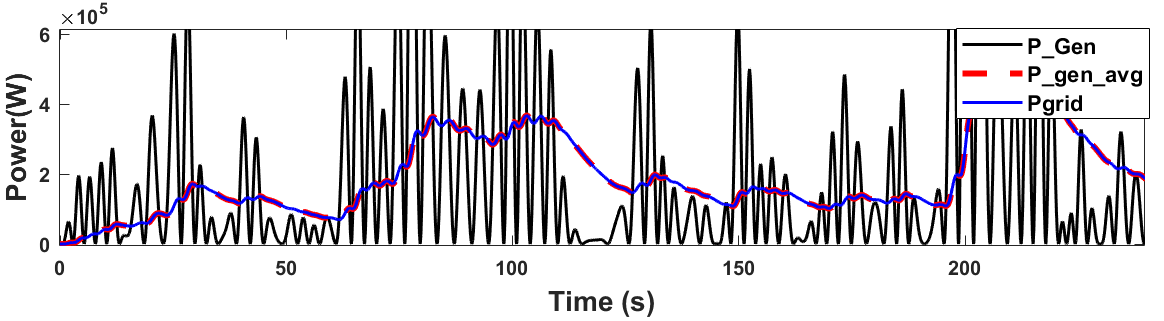
\includegraphics[width=0.5\textwidth]{Figs/5_3_1/power all.png}
    \caption{Generated power from LPMG, power after smoothing out, grid injected power.}
    \label{fig:W2G_normal_grid}
\end{figure}

\begin{figure}[h!]
    \centering
    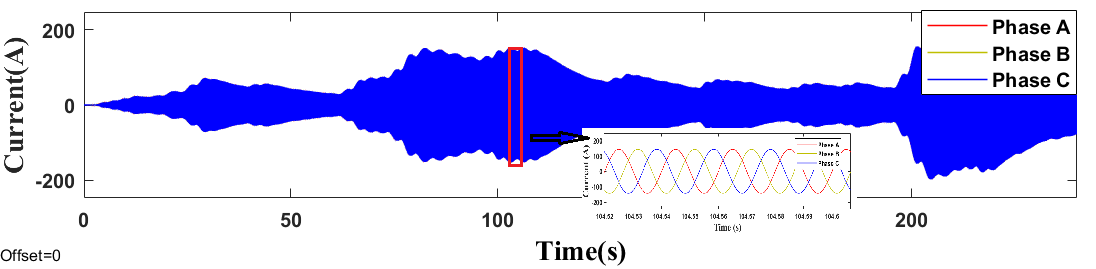
\includegraphics[width=0.5\textwidth]{Figs/5_3_1/grid current merged.png}
    \caption{Grid injected current  }
    \label{fig:LPMG_position_velocity}
\end{figure}

\subsection{Grid Fault Condition}
During a fault, low voltage or voltage sag occurs at the point of common connection (PCC). The depth of voltage sag depends on the severity of the grid fault. As mentioned above, grid code requires an inverter-based generation to ride through the voltage sag for a certain amount of time and also inject reactive current to improve the voltage. The three-phase fault is the most severe type of fault that may occur in the grid. Thus, three-phase faults of different voltage sag levels are applied to the grid at different times to examine the performance of the W2G system during fault.

The performance of the W2G system in the case of symmetrical faults is shown in Fig. 9-14. At 8s, the voltage dip at the PCC is 0.7 p.u. As \( \frac{v_d^p}{v_{\text{nominal}}} < 0.5 \), the W2G system stops supplying active current into the grid while starting to inject reactive current at the converter’s full rated value. Fig. 11-12 shows the d-, q- and 3-phase currents during the fault duration of 8s-8.9s. Active and reactive power supply to the grid during the fault time is shown in Fig. 13-14. However, the Gen-SC continues to extract the maximum power from wave resources, as shown in Fig. 13. DC bus voltage fluctuates due to the power mismatch, and this difference of power continues to be stored in the SC until the fault is cleared. The controller is designed to track the mismatched energy and release that energy to the grid after the fault clearance. For that reason, the injected grid power is higher than the generated power from 8.9s to 10.3s, the time required to release all the stored mismatch energy.
\begin{figure}[htbp]
    \centering
    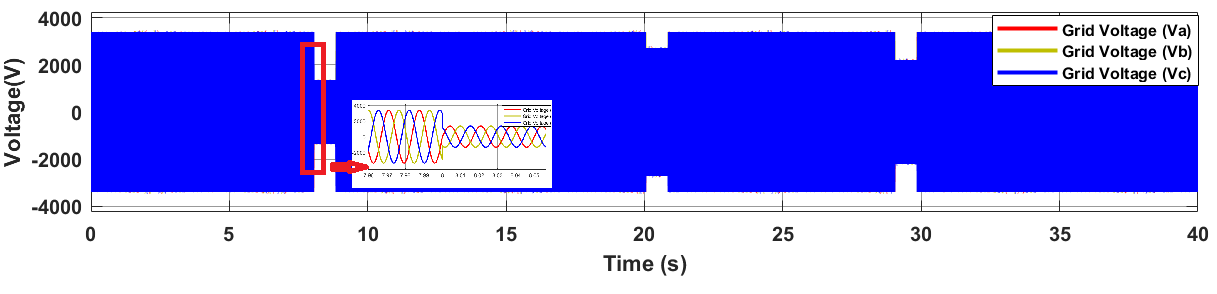
\includegraphics[width=0.5\textwidth]{Figs/5_3_1/voltage abc.png}
    \caption{Three-phase grid voltage}
    \label{fig:W2G_normal_grid}
\end{figure}
\begin{figure}[h!]
    \centering
    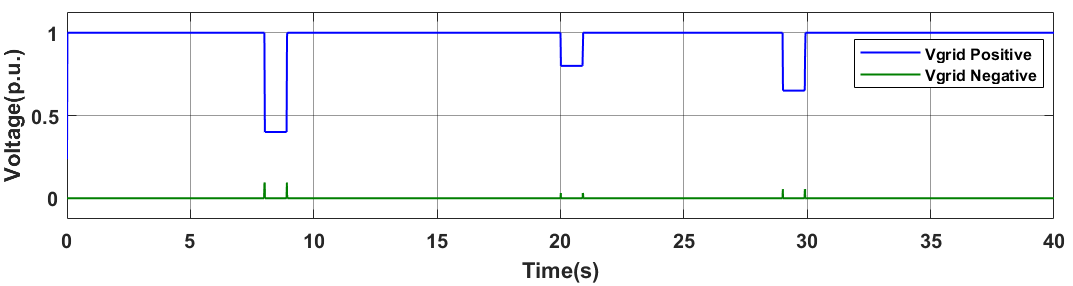
\includegraphics[width=0.5\textwidth]{Figs/5_3_1/voltage pu.png}
    \caption{Voltage p.u. magnitude.}
    \label{fig:LPMG_position_velocity}
\end{figure}
\begin{figure}[h!]
    \centering
    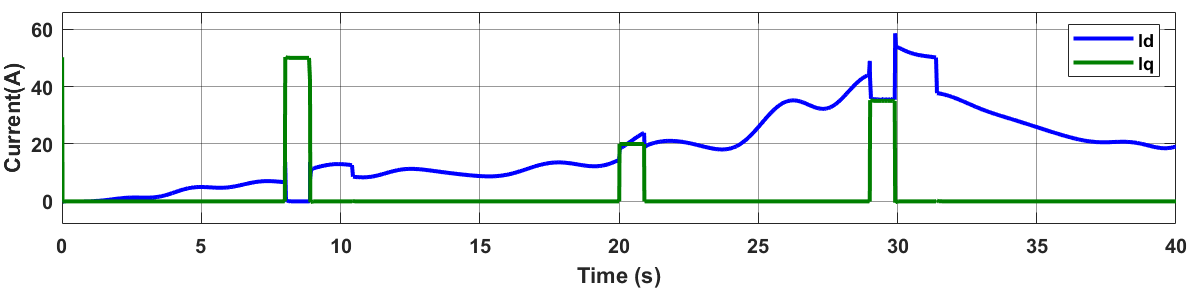
\includegraphics[width=0.5\textwidth]{Figs/5_3_1/idq.png}
    \caption{: d- and q- axis current out of Grid-SC}
    \label{fig:W2G_normal_grid}
\end{figure}

\begin{figure}[h!]
    \centering
    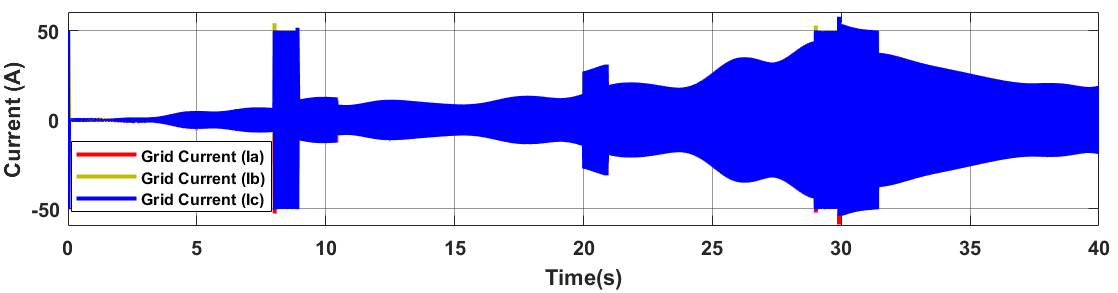
\includegraphics[width=0.5\textwidth]{Figs/5_3_1/current.png}
    \caption{Three-phase current output}
    \label{fig:LPMG_position_velocity}
\end{figure}
\begin{figure}[h!]
    \centering
    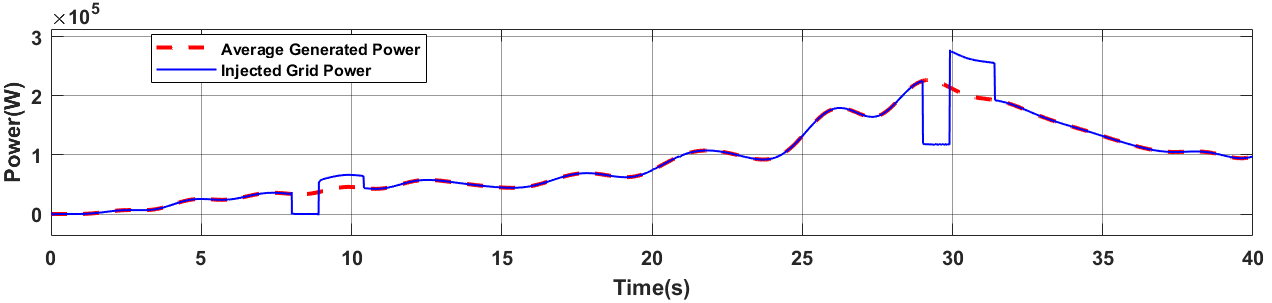
\includegraphics[width=0.5\textwidth]{Figs/5_3_1/active power lvrt.png}
    \caption{Generated active power and injected grid active power.}
    \label{fig:W2G_normal_grid}
\end{figure}

\begin{figure}[h!]
    \centering
    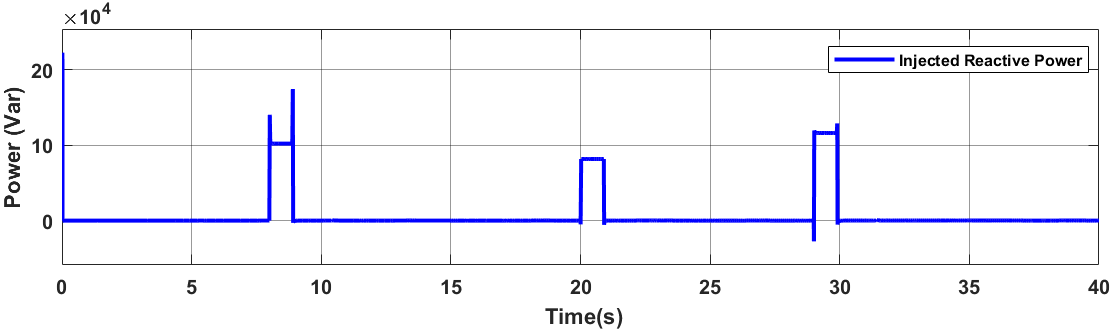
\includegraphics[width=0.5\textwidth]{Figs/5_3_1/reactive power lvrt.png}
    \caption{Grid injected reactive power .}
    \label{fig:LPMG_position_velocity}
\end{figure}

Another three-phase fault is simulated at 20s with a voltage sag of 0.8 p.u. at the PCC. As \( \frac{v_d^p}{v_{\text{nominal}}} > 0.5 \), the W2G system supplies both active and reactive current according to equation (15). In this case, the reactive current reference, as well as the reactive power reference, is obtained from the grid code requirement. Active current (power) injection during the fault follows the generated power because the inverter output current with the desired reactive current and active current remains below the maximum current limit, as shown in Fig. 12. So, for this fault sag, there is no mismatch between the generated and injected power.

Finally, another symmetrical fault is simulated with a voltage sag of 0.65 p.u. Both the active and reactive current will be injected in this case. However, unlike the previous fault case, here, the injected grid power reference does not follow the generated power as the current exceeds the maximum limit of the inverter to supply all the generated power and the reactive power required by the grid code. So, the current limiting control strategy becomes activated, which reduces the active power reference to its maximum allowable value, avoiding the inverter current limit violation. This scenario is shown in Fig. 12-13. The mismatch power remains stored in SC and gets released as the fault clears.
\begin{figure}[htbp]
    \centering
    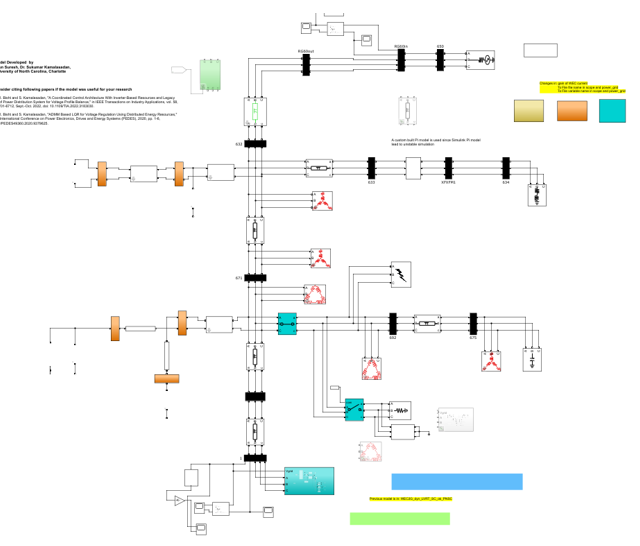
\includegraphics[width=0.5\textwidth]{Figs/5_3_1/13 bus.png}
    \caption{13-bus distribution network.}
    \label{fig:W2G_normal_grid}
\end{figure}
\begin{figure}[h!]
    \centering
    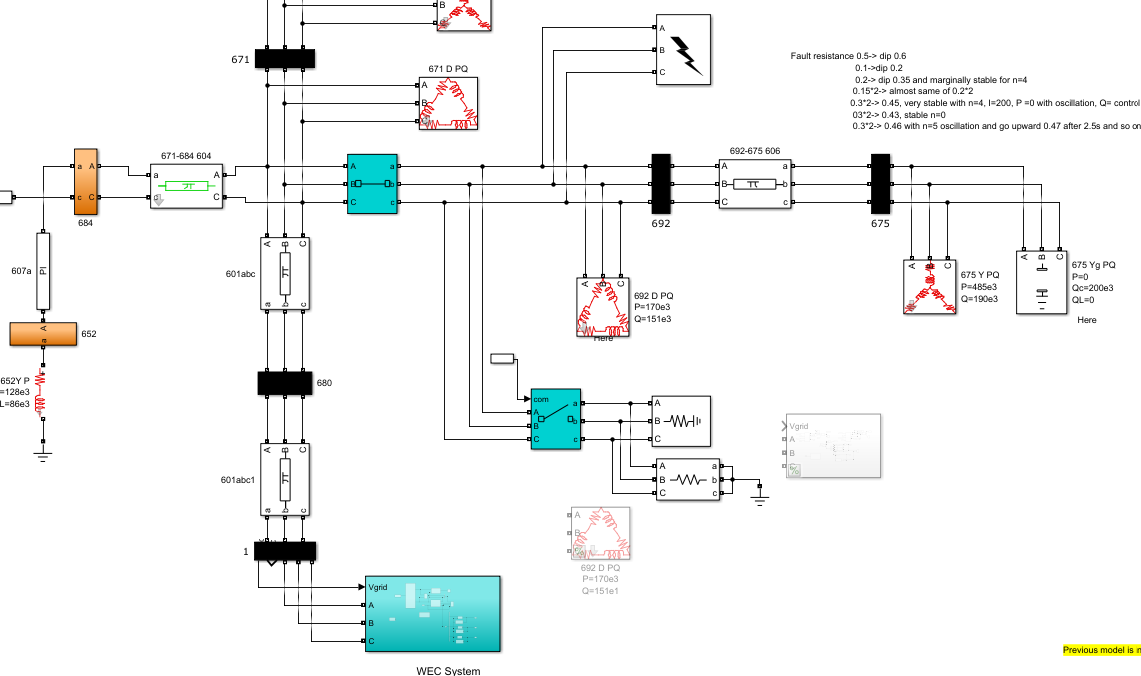
\includegraphics[width=0.5\textwidth]{Figs/5_3_1/wec connection 13 bus.png}
    \caption{WEC system connection to bus 680.}
    \label{fig:W2G_normal_grid}
\end{figure}


\subsection{Effect of Distribution Network}
The W2G system is connected to an IEEE 13-node test feeder to investigate the effect of variable power wave energy on the distribution system parameters. System parameters like voltage and frequency behavior have been observed. The W2G system is connected to a remote 3-phase bus, bus 680, in the distribution network with a connecting feeder length of 1 km shown in Fig. 15-16.


\subsubsection{Effect on Voltage}
The IEEE 13-node feeder is an unbalanced system. The voltage at each phase becomes more unbalanced as it becomes away from the connected grid. Also, not all the 13 buses are 3-phase buses. A regulator is used to improve the voltage profile of the distribution feeder. In the IEEE 13 bus benchmark system, the regulator is connected between buses 650 and 632. Fig.17-19 shows the voltage profile of each phase of bus 680 with different penetration levels of wave energy generation. \\

\begin{figure}[htbp]
    \centering
    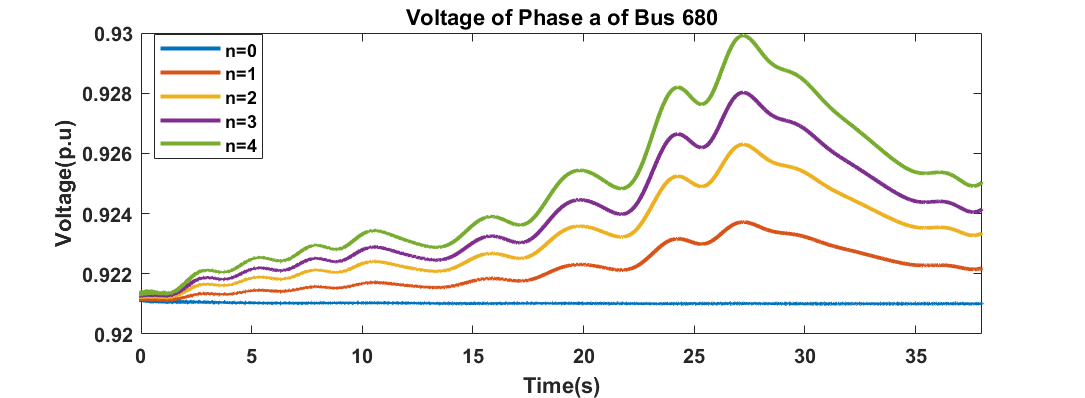
\includegraphics[width=0.5\textwidth]{Figs/5_3_1/vol_normal680a.png}
    \caption{Voltage of Phase a of Bus 680.}
    \label{fig:W2G_normal_grid}
\end{figure}
\begin{figure}[h!]
    \centering
    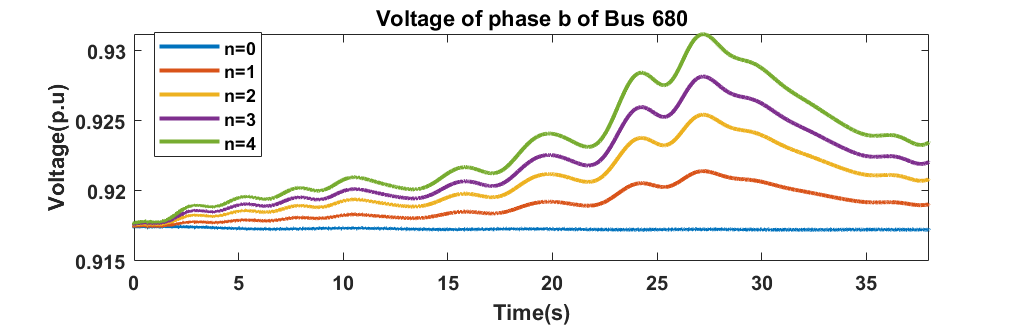
\includegraphics[width=0.5\textwidth]{Figs/5_3_1/vol_normal680b.png}
    \caption{Voltage of Phase b of Bus 680.}
    \label{fig:LPMG_position_velocity}
\end{figure}
\begin{figure}[h!]
    \centering
    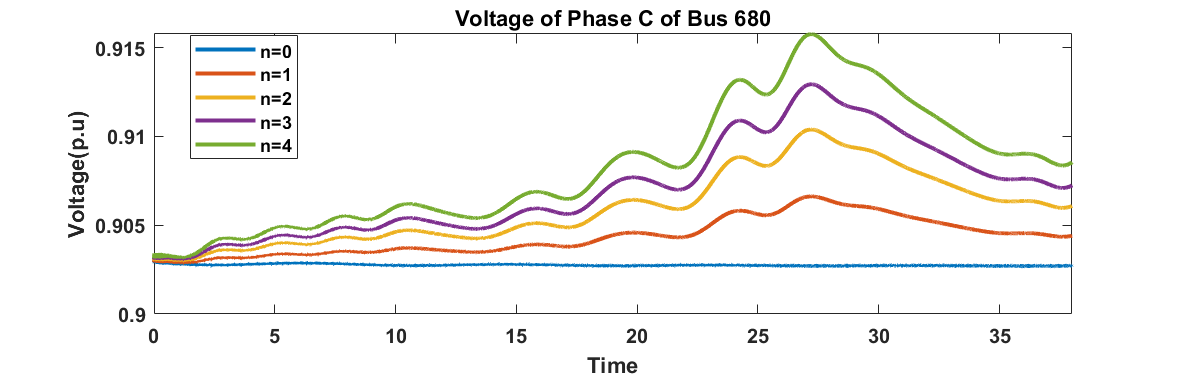
\includegraphics[width=0.5\textwidth]{Figs/5_3_1/vol_normal680c.png}
    \caption{Voltage of Phase c of Bus 680.}
    \label{fig:W2G_normal_grid}
\end{figure}

\begin{figure}[h!]
    \centering
    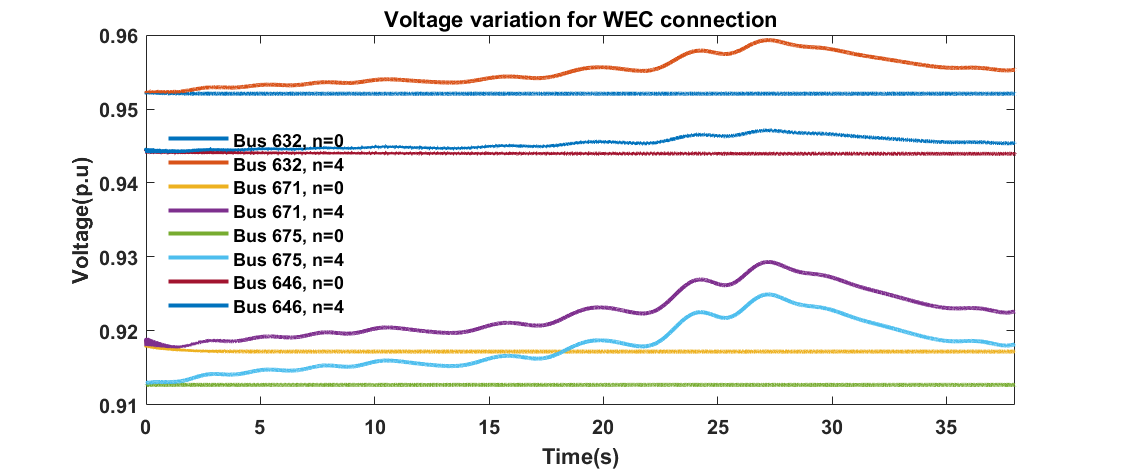
\includegraphics[width=0.5\textwidth]{Figs/5_3_1/various bus.png}
    \caption{Effect of variable WECs power on  the voltage of different buses.}
    \label{fig:LPMG_position_velocity}
\end{figure}

 As the penetration level increases, the voltage magnitude increases. The voltage magnitude for other buses also increases after adding the W2G system. Fig.20 shows the phase voltage of bus 632, 671, 675, and 646 before and after the addition of the W2G system. However, the voltage profile shows fluctuations after adding the variable output wave generation. This fluctuation can be mitigated by smoothing out the output power variation from WEC or by creating a WEC farm by optimally spacing individual WEC to smooth out the total output power from the farm.\\
 
The voltage profile during fault is also investigated. At 10s, a 3-phase impedance fault is applied to the grid. The voltage profile of bus 680 due to fault is shown in Fig 21-22 before and after the addition of the W2G system. The W2G system injects reactive power to support the voltage profile during low voltage. As the penetration level increases, the minimum voltage depth reduces. This scenario indicates that the W2G system is beneficial in reducing the fault effect on the distribution grid.  As the fault is initiated, the active power supply to the network from the W2G system reduces, and reactive power injections start. The W2G system returns to its normal pre-fault operation after the fault clearance. 
\begin{figure}[htbp]
    \centering
    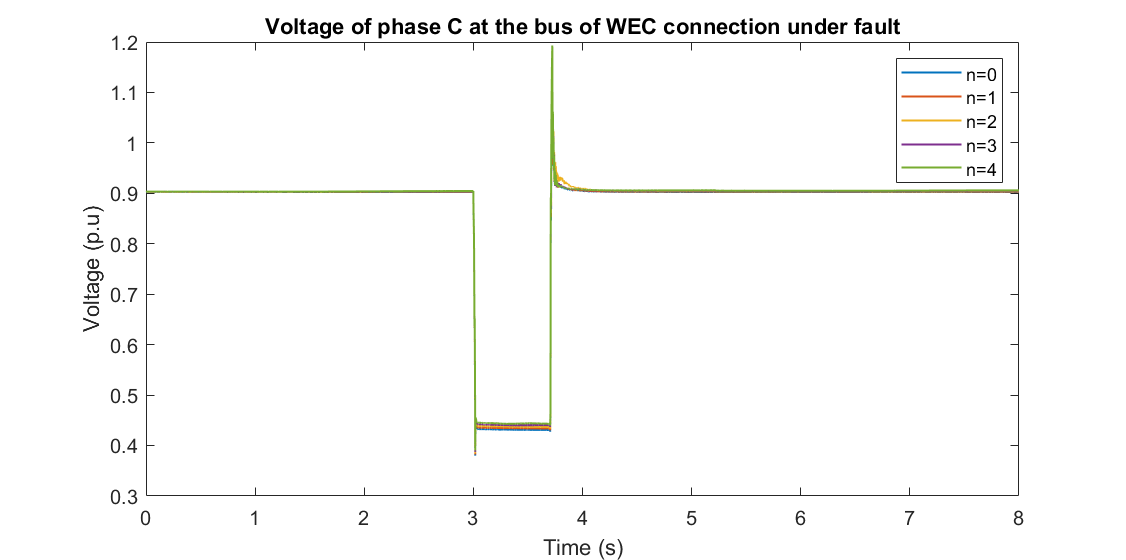
\includegraphics[width=0.5\textwidth]{Figs/5_3_1/Vol dis fault.png}
    \caption{Voltage profile at PCC during fault}
    \label{fig:W2G_normal_grid}
\end{figure}
\begin{figure}[h!]
    \centering
    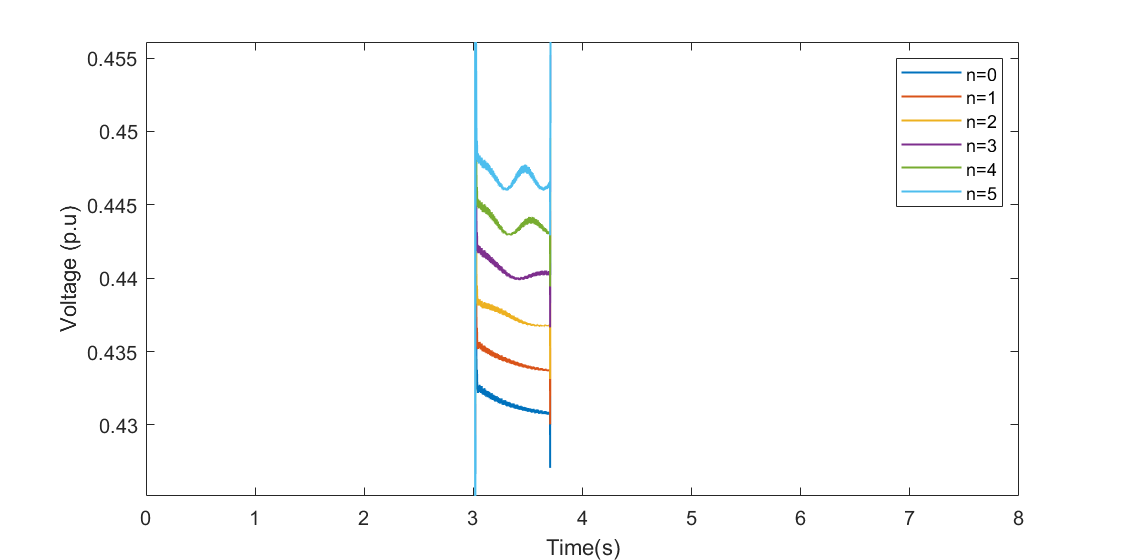
\includegraphics[width=0.5\textwidth]{Figs/5_3_1/Vol dis fault zoomed1.png}
    \caption{zoomed view of voltage profile at PCC during fault}
    \label{fig:W2G_normal_grid}
\end{figure}
\subsubsection{Effect on Frequency}
The frequency of a system is determined by the balance between active power demand and generation. When the active power demand exceeds the available generation, the system frequency decreases, and conversely, when generation exceeds demand, the frequency increases. Fig.23 illustrates the frequency of the studied 13-node system both before and after the integration of wave energy generation. The system frequency remains relatively stable, showing no significant deviations regardless of the level of wave energy penetration. This stability is attributed to the fact that, as wave energy penetration increases, the power supplied by the grid decreases proportionately, as depicted in Fig.24. Therefore, the impact of adding variable power from wave energy to the distribution network under normal grid conditions is minimal.
\begin{figure}[htbp]
    \centering
    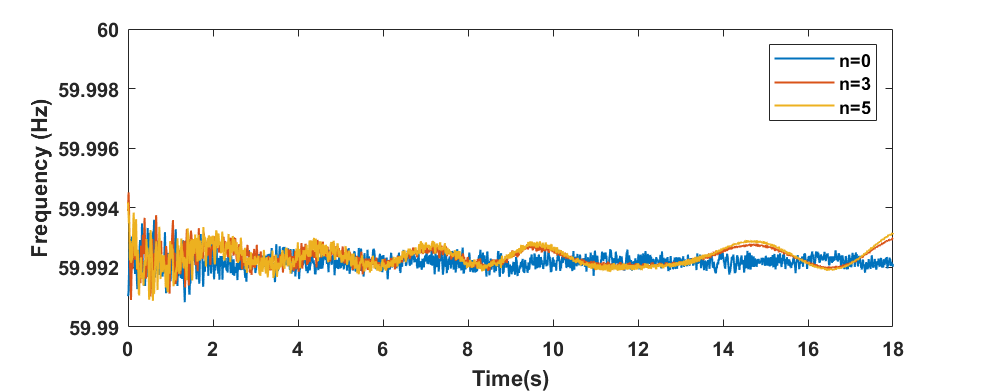
\includegraphics[width=0.5\textwidth]{Figs/5_3_1/frequency.png}
    \caption{Effect of variable WECs on system frequency}
    \label{fig:W2G_normal_grid}
\end{figure}
\begin{figure}[h!]
    \centering
    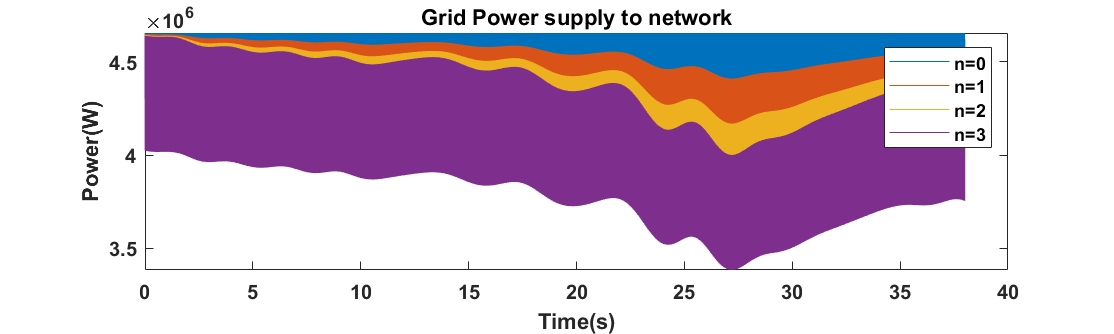
\includegraphics[width=0.5\textwidth]{Figs/5_3_1/grid power.png}
    \caption{Grid power supply variation.}
    \label{fig:W2G_normal_grid}
\end{figure}

\section{Conclusion}

This report presents the development of LVRT capability for the grid-side converter in the studied W2G system. It includes a detailed mathematical model for LVRT control and demonstrates the performance of the WEC system during grid-side faults. Furthermore, the impact of integrating variable power wave generation into an unbalanced distribution network is analyzed to evaluate the voltage and frequency stability of a test system.

\begin{thebibliography}{6}

\bibitem{NREL}
National Renewable Energy Laboratory (NREL), “Marine Energy Basics,” available: \url{https://www.nrel.gov/research/marine-energy.html}. [Accessed: Jun. 21, 2024].

\bibitem{EirGrid}
EirGrid, “Grid Code, Version 6.0,” Technical report, EirGrid, 2015.

\bibitem{Tsili}
M. Tsili and S. Papathanassiou, “A review of grid-code technical requirements for wind farms,” \textit{IET Renew. Power Gener.}, vol. 3, no. 3, pp. 308–332, 2009.

\bibitem{Lu}
S. Lu, L. Wang, T.-M. Lo, and A. V. Prokhorov, “Integration of wind power and wave power generation systems using a DC microgrid,” \textit{IEEE Trans. Ind. Appl.}, vol. 51, no. 4, pp. 2753–2761, Jul./Aug. 2015.

\bibitem{Wang1}
L. Wang, C.-Y. Lin, H.-Y. Wu, and A. V. Prokhorov, “Stability analysis of a microgrid system with a hybrid offshore wind and ocean energy farm fed to a power grid through an HVDC link,” \textit{IEEE Trans. Ind. Appl.}, vol. 54, no. 3, pp. 2012–2022, May/Jun. 2018.

\bibitem{Wang2}
L. Wang, H.-W. Li, and C.-T. Wu, “Stability analysis of an integrated offshore wind and seashore wave farm fed to a power grid using a unified power flow controller,” \textit{IEEE Trans. Power Syst.}, vol. 28, no. 3, pp. 2211–2221, Aug. 2013.
\bibitem{wu}
F. Wu, X. Zhang, P. Ju, and M. J. H. Sterling, ``Modeling and Control of AWS-Based Wave Energy Conversion System Integrated Into Power Grid'', \textit{IEEE Trans. on Power Sys.}, vol. 23, no. 3, pp. 1196-1204, August 2008.

\end{thebibliography}



\end{document}
